%% In the documentclass line, replace "noanswers" with "answers" to view the key.

\documentclass[noanswers]{exam}
\usepackage[utf8]{inputenc}

\title{Chapter 2 Practice Problems}
\author{Sections 2.1--2.2}
\date{STAT 2300}

\usepackage[bottom=2.2cm, left=2.2cm, right=2.2cm, top=2.2cm]{geometry}
%\usepackage[paperheight=11in, paperwidth=17in, margin=1in]{geometry}
\usepackage{dsfont}
\usepackage{amsmath}
\usepackage{amssymb}
\usepackage{amsthm}
\usepackage{array}
\usepackage{stmaryrd}
\usepackage{pgfplots}
\pgfplotsset{width=10cm,compat=1.9}
\usepackage{multicol}
\setlength{\columnsep}{1in}
\usepackage{nicefrac}

\usepackage{multirow}
\usepackage{enumitem}[shortlabels]
\usepackage{tabu}
\definecolor{purp}{RGB}{102,0,204}
\usepackage{tabularx}
\newcolumntype{C}{>{\centering\arraybackslash $}X<{$}}
\usepackage{wrapfig}
\usepackage[export]{adjustbox}


\makeatletter
\pagestyle{headandfoot}
\firstpageheader{\@date}{\@title}{\@author}
\firstpageheadrule
\runningfootrule
\runningfooter{}{\thepage\ / \numpages}{\@title}
\makeatother

\newcommand{\abs}[1]{\left|#1\right|}
\newcommand{\mat}[4]{\left( \begin{tabular}{>{$}c<{$} >{$}c<{$}} #1&#2 \\ #3&#4 \end{tabular} \right)}
\newcommand{\msc}[1]{\mathds{#1}}
\newcommand{\Z}{\mathds{Z}}
\newcommand{\R}{\mathds{R}}
\newcommand{\N}{\mathds{N}}
\newcommand{\Q}{\mathds{Q}}
\newcommand{\C}{\mathds{C}}
\newcommand{\so}{\implies}
\newcommand{\set}[2]{\left\{ #1 \:|\: #2 \right\}}
\newcommand{\bso}{\Longleftarrow}
\newcommand{\ra}{\rightarrow}
\newcommand{\gen}[1]{\left\langle #1 \right\rangle}
\newcommand{\olin}[1]{\overline{#1}}
\newcommand{\Img}[1]{\text{Im}\left(#1\right)}
\newcommand{\llra}{\longleftrightarrow}
\newcommand{\lra}{\longrightarrow}
\newcommand{\xra}[1]{\xrightarrow{#1}}
\newcommand{\wo}{\setminus}
\newcommand{\mcal}[1]{\mathcal{#1}}
\newcommand{\Aut}[1]{\text{Aut}\left(#1\right)}
\newcommand{\Inn}[1]{\text{Inn}\left(#1\right)}
\newcommand{\syl}[2]{\text{Syl}_{#1}(#2)}
\newcommand{\norm}[1]{\left\|#1\right\|}
\newcommand{\infnorm}[1]{\left\|#1\right\|_{\infty}}
\newcommand{\xn}{\{x_n\}}
\newcommand{\sig}{\sigma}
\newcommand{\id}{\text{id}}
\newcommand{\ep}{\epsilon}
\newcommand{\st}{\text{ s.t. }}
\newcommand{\ran}[1]{\text{Ran}(#1)}
\newcommand{\nCr}[2]{\binom{#1}{#2}}
\newcommand{\Exr}[1]{\paragraph{Exercise #1:}}
\newcommand{\pg}{\paragraph{}}
\newcommand{\ulin}[1]{\underline{#1}}
\newcommand{\tc}[1]{\textcolor{purp}{#1}}

% Solution Specs
\unframedsolutions
\renewcommand{\solutiontitle}{}
\SolutionEmphasis{\color{purp}}
\CorrectChoiceEmphasis{\color{purp}\bfseries}
\setlength\fillinlinelength{0in}

\renewcommand{\arraystretch}{2}


%\begin{solution}[\stretch{1}]
%	hurp durp flurp
%\end{solution}

%\pagestyle{empty}

\begin{document}
%\noindent\begin{tabular}{@{}p{.3in}p{3in}@{}}
%Name: & \hrulefill
%\end{tabular}

\begin{questions} 

	\question You take a look around your classroom one day and note what color shirts your classmates are wearing, collecting the following data.  
	
	\begin{center}
    \begin{tabular}{c c c c c c c c c c}
        Purple & Blue & Black & Purple & Blue & Black & Pink & Purple & Purple & Red\\   
        Black & Blue & Orange & Orange & Blue & Red & Orange & Pink & White & Purple\\  
        Green & Orange & White & Purple & Black & Yellow & Green & Red & Pink & Orange \\
    \end{tabular}
\end{center}
	
	\vspace{3mm}
	
	Use the data collected to construct a \textbf{frequency} and \textbf{relative frequency} distribution.

\begin{center}
\begin{tabular}{|*{3}{c|}}
\hline
\textbf{Color} & \textbf{Frequency} & \textbf{Relative Frequency}\\
\hline
Red & \fillin[3] & \fillin[$\frac{3}{30} = 0.100$] \\ 
\hline
Orange & \fillin[5] & \fillin[$\frac{5}{30} = 0.167$] \\
\hline
Yellow & \fillin[1] & \fillin[$\frac{1}{30} = 0.033$] \\
\hline
Green & \fillin[2] & \fillin[$\frac{2}{30} = 0.067$] \\
\hline
Blue & \fillin[4] & \fillin[$\frac{4}{30} = 0.133$] \\
\hline
Purple & \fillin[6] & \fillin[$\frac{6}{30} = 0.200$] \\
\hline
Pink & \fillin[3] & \fillin[$\frac{3}{30} = 0.100$] \\
\hline
Black & \fillin[4] & \fillin[$\frac{4}{30} = 0.133$] \\
\hline
White & \fillin[2] & \fillin[$\frac{2}{30} = 0.067$] \\
\hline
Total & \fillin[30] & \fillin[$\frac{30}{30}=1.00$] \\
\hline
\end{tabular}
\end{center}

\vspace{3mm}

\newpage

\question Consider the following scores that Miss Frizzle's students made on their Biology final exam.
	
	\begin{center}
    \begin{tabular}{c c c c c c c c c c c c c c c c}
        51 & 57 & 59 & 62 & 64 & 65 & 65 & 68 & 71 & 72 & 74 & 78 & 78 & 78 & 79 & 80\\   
        83 & 83 & 85 & 86 & 87 & 87 & 87 & 89 & 89 & 90 & 91 & 93 & 93 & 94 & 95 & 97\\  
        97 & 98 & 98 & 99 & 100\\
    \end{tabular}
\end{center}

\vspace{1mm}

Construct a \textbf{stem-and-leaf plot} of the exam scores. Include a \textbf{key}.

\begin{solution}[\stretch{5}]
	
			Key: 5 $|$ 1 = exam score of 51		
		
			\vspace{3mm}
		
			\begin{tabular}{r|l}
			5 & 1 7 9 \\
			6 & 2 4 5 5 8\\ 
			7 & 1 2 4 8 8 8 9\\
			8 & 0 3 3 5 6 7 7 7 9 9\\
			9 & 0 1 3 3 4 5 7 7 8 8 9\\
			10 & 0			
			\end{tabular}

			\vspace{2mm}		
			
		\end{solution}
		
\question Consider the following histogram of waiting times (in minutes) for a sample of 170 patients at Grey Sloan Memorial Hospital.

\begin{center}
	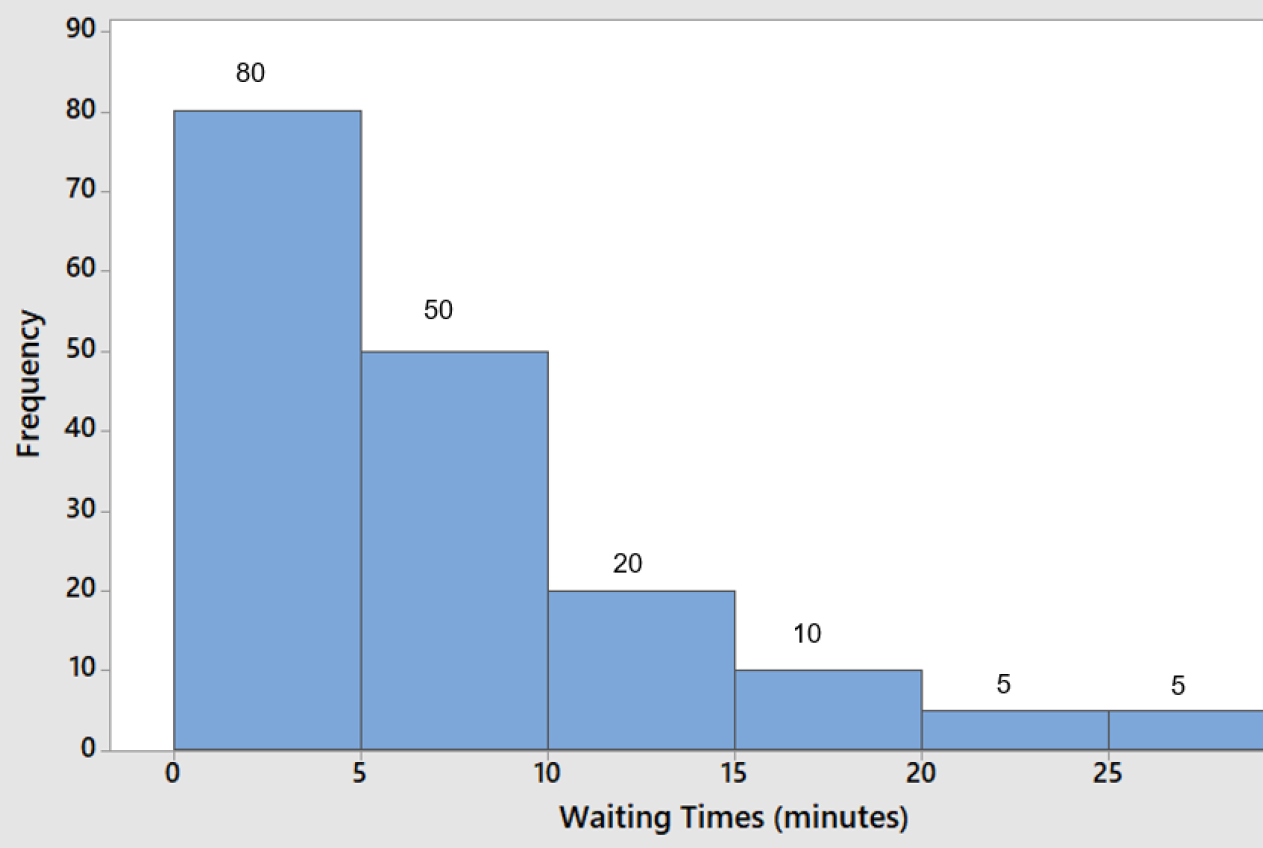
\includegraphics[scale=.18]{STAT_2300_Practice_2-1_2-2_histogram.png}
\end{center}

\begin{parts}
	
	\part Describe the \textbf{shape} of the distribution.
	
	\begin{solution}[\stretch{1}]
	
			\vspace{1mm}		
		
			The distribution is skewed right, with most of the values clustering in the 0--10 minute range. There are no gaps or clear outliers in the data.

			\vspace{1mm}		
			
		\end{solution}
		
	\part What \textbf{class width} was chosen for the histogram? (Include units in your answer.)
	
	\begin{solution}[\stretch{1}]
	
			\vspace{1mm}		
		
			The class width is 5 minutes.

			\vspace{1mm}		
			
		\end{solution}
	
	\part How many patients had to wait \textbf{longer than} twenty minutes?
	
	\begin{solution}[\stretch{1}]
	
			\vspace{1mm}		
		
			10 patients had to wait longer than 20 minutes. (Add the frequencies from the 20--25 and 25--30 classes.)

			\vspace{1mm}		
			
		\end{solution}
		
	\part What is the \textbf{relative frequency} of patients who waited less than five minutes?
	
	\begin{solution}[\stretch{.5}]

			\vspace{1mm}		
			
			$\displaystyle \frac{80}{170} \approx 0.471$ (47.1\%) of patients waited less than 5 minutes.
		\end{solution}
	
\end{parts}


\end{questions}

%-----------------------------------------------------------------------------%

\end{document}
